% !TEX spellcheck = en_US
% Tower Damper
%=================================================================================
This section describes the the function and the implementation of a pitch angle based Tower Damper (TD). !!! Abbreviation package !!! The design follows the description in \cite{WindEnergyHandbook} similar as the workflow in the exercise of the corresponding lecture and lecture notes \cite{2024}. The tower dynamics are modeled as in \cite{WindEnergyHandbook} (eq: 8.12 and 8.13). Here referd as \ref{eq:TowerDynamics} and \ref{eq:TowerDamper}.
\begin{equation}
	M\ddot{x} + D\dot{x} + Kx = F + \Delta F
	\label{eq:TowerDynamics}
\end{equation}
\begin{equation}
	\begin{aligned}
		\Delta F = \frac{\partial F}{\partial \theta}\Delta\theta = -D_{\text{TD}}\dot{x}\\
		\Delta\theta = \frac{-D_{\text{TD}}}{\partial F/\partial \theta}\dot{x}
	\end{aligned}
	\label{eq:TowerDamper}
\end{equation}
As described by equation \ref{eq:TowerDynamics} the dynamics of the tower in fore-aft direction are lightly damped if $D$ is small and the force $\Delta F$ which is the additional thrust force resulting of a pitch action is equal to zero. The force $F$ is damped by the relative wind speed $v_{\text{rel}} = v_0 - \dot{x}$ and therefore $F = F(\Omega, \theta, v_{\text{rel}})$ \cite{2024}. To damp the tower top speed $\dot{x}$ even further \cite{WindEnergyHandbook} proposes an update of the pitch angle of $\Delta\theta$. This will damp the tower motion further as described in \ref{eq:TowerDamper}. This lead to a reduction of the tower bottom bending moment. Nevertheless this comes at a cost of higher pitch activity and the damping is only available in control region 3. The static tower top deflection over the regions are shown in section \ref{steady states}. This is helpful to see when the damper is active and what can be damped. 

The implementation and test of the damper is done in Matlab and Simulink. As in the lecture and the corresponding exercise \cite{2024} the tower top acceleration $\ddot{x}$ is measured in reality. To make the simulation task as similar to a real world application here also the the tower top acceleration is used. What is also taken into account is the existence of a real pitch actuator. This means that the pitch update $\Delta\theta$ can not be applied instantaneously because of the time constants of the pitch actuator. To address this phenomena there are 2 methods tested. First a direct integration \ref{eq:TDintegration}: 
\begin{equation}
	\dot{x}(t) = \int\ddot{x}(t) \text{d}t
	\label{eq:TDintegration}
\end{equation} 
And second a phase shift of $90^{\circ}$ of the speed signal by a Lag-Compensator. The Transferfunction in the frequency domain is shown in equation \ref{eq:LagCompensator}. Where the input in the frequency domain is $\ddot{X}$ and the output is $\dot{X}$. 
\begin{equation}
	\frac{\ddot{X}(s)}{\dot{X}(s)} = \frac{s + z}{s + p}
	\label{eq:LagCompensator}
\end{equation} 
\begin{equation}
	\dot{x}(t) = \ddot{x}(t) - \int p\dot{x}(t) - z\ddot{x}(t) \text{d}t
	\label{eq:xddTimeDomain}
\end{equation} 

% explain analytical why this should work better

The implementation in Simulink is first following the approach in the exercise \cite{2024}.
\begin{figure}[tbh]
	\centering	
	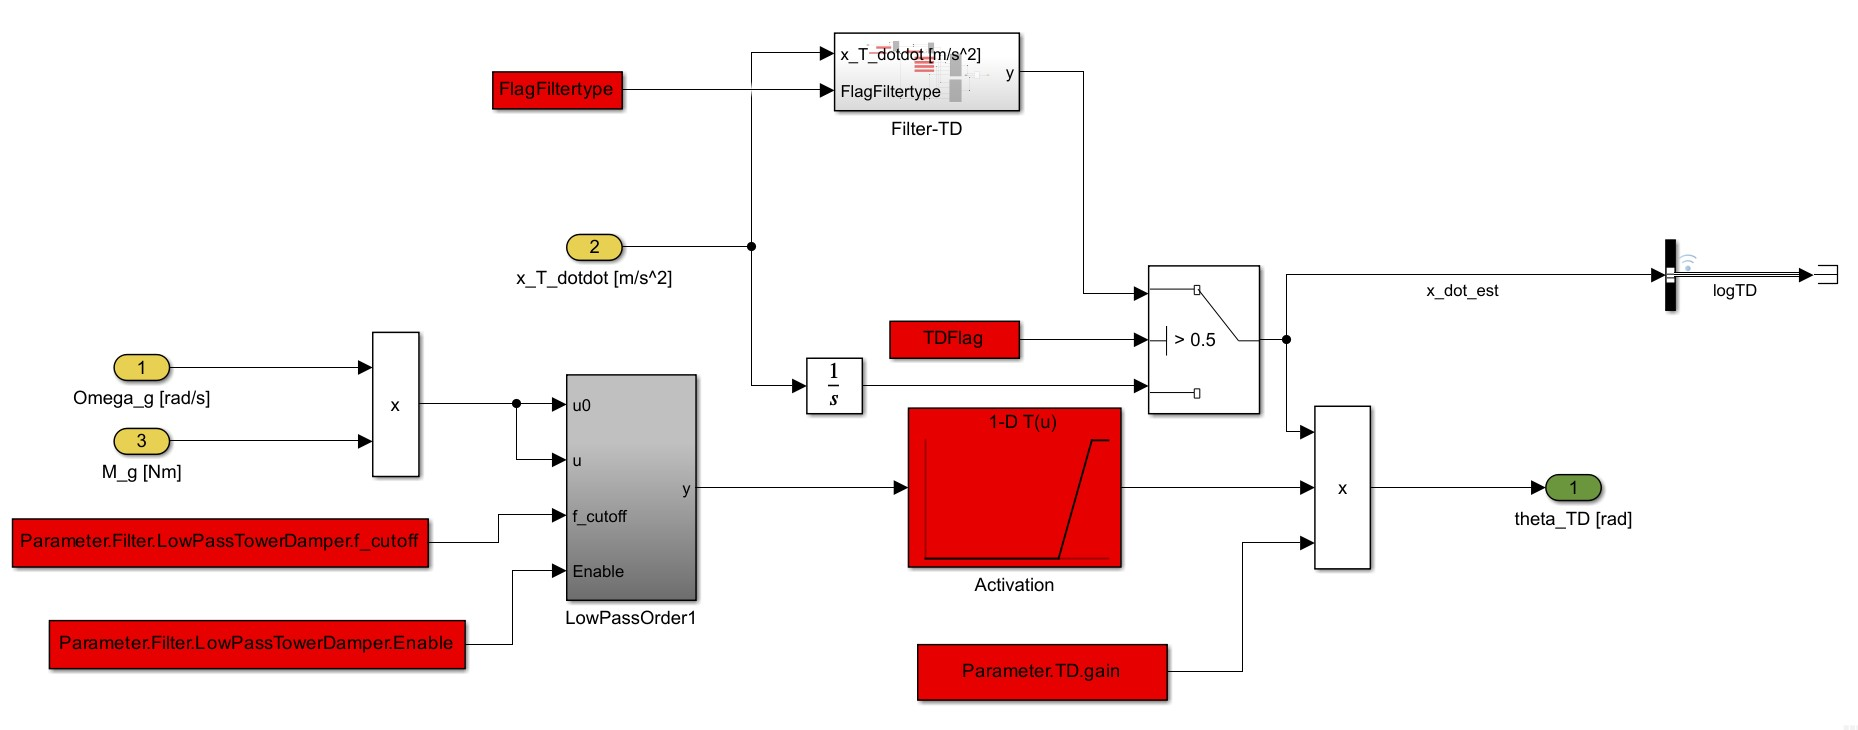
\includegraphics[width=12cm]{Figures/TDoverview}
	\caption{Tower Damper in Simulink model}
	\label{fig:TDoverview}
\end{figure}  
The input \textit{Omega\_g} is already a filtered value. It is low pass filtered and the 3P blade passing frequency is notched. As shown in figure \ref{fig:TDoverview} to activate the TD the generator power is used. The \textit{LowPassOrder1} is used to reduce the switching frequency of the TD to ensure that it is not switched on and of if the WT is operating near rated conditions. In the activation the gain is slowly ramped up from $\SI{0}{\%}$ to $\SI{100}{\%}$ over a power range from $\SI{80}{\%}$ of the rated power to $\SI{100}{\%}$ and stays there. 

In the first method, here named integrator, the tower top acceleration signal is integrated and than multiplied with the damping gain \textit{Parameter.TD.gain} and the activation signal as shown in figure \ref{fig:TDoverview}. The resulting quantity is the pitch offset mentioned in equation \ref{eq:TowerDamper}. This offset $\Delta\theta$ is added to the pitchangle control value of the collective-pitch-controller and this together is the new input for the pitch actuator od the SLOW-model.

The second method, here named Lag-Compensator, isolates the tower eigenfrequency by passing the acceleration signal first through a low pass filter and than a high pass filter. The cutoff frequency of the low pass filter is above the eigenfrequency of the tower and the cutoff frequency of the high pass filter is below the eigenfrequency. Now the signal contains mainly the isolated eigenfrequency of the tower with which the tower is oscillating in the fore-aft direction. To phase shift the signal a lag compensator is used. 
\begin{figure}[tbh]
	\centering	
	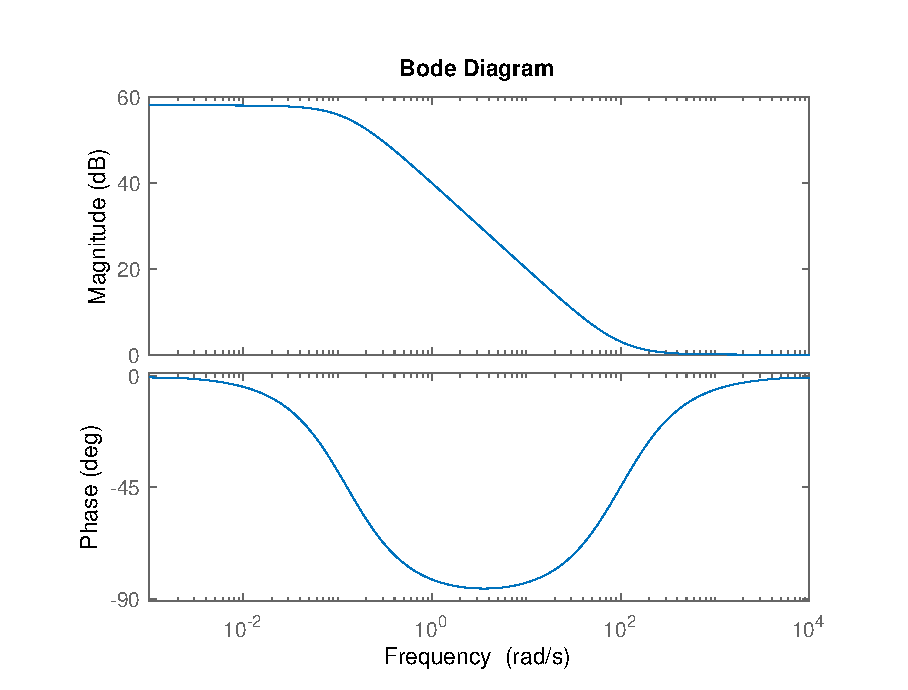
\includegraphics[width=12cm]{Figures/BodeLagCompensator.eps}
	\caption{Bode plot of the Lag-Compensator}
	\label{fig:BodeLag}
\end{figure} 
\begin{figure}[tbh]
	\centering	
	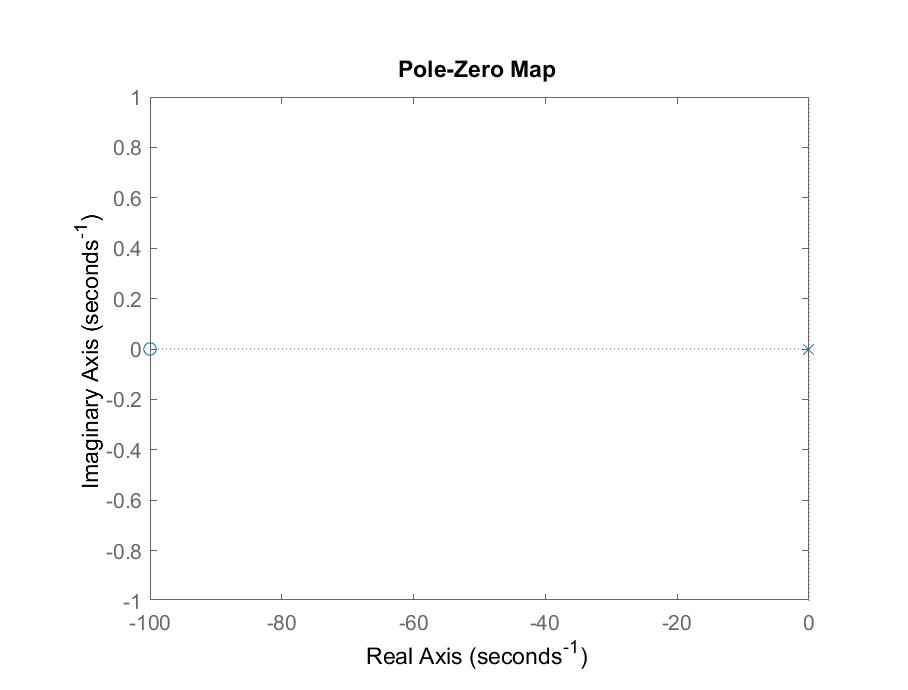
\includegraphics[width=12cm]{Figures/PoleZeroMapLagCompensator.eps}
	\caption{Pole-Zero-Map of the Lag-Compensator}
	\label{fig:ZeroPoleLag}
\end{figure} 
As shown in figure \ref{fig:BodeLag} the frequency that has been isolated by the previous filters is phase shifted by nearly $90^{\circ}$ and the magnitude of this frequency is increasing by $\SI{30}{dB}$. The increase in magnitude and the general difference in magnitude of the $\ddot{x}(t)$ signal compared to the $\dot{x}(t)$ can be achieved by a different gain value which will result in a similar damping behavior. Figure \ref{fig:ZeroPoleLag} shows the Pole-Zero-Map of the Lag-Compensator. The $\color{blue} \circ$ shows the zero and the $\color{blue} \times$ shows the pole. the zero $z = -100$ and the pole $p = -0.125$ in the shown plot.

The design is tested first with a wind step from $v_0 = \SI{20}{m/s}$ to $v_1 = \SI{21}{m/s}$ to ensure the general functionality of the methods shown in figure \ref{fig:TDWindStepEst}. The figure shows the acceleration reference value, both speed estimation methods need to be $90^{\circ}$ phase shifted compared to this signal. The figure shows the estimated speeds after the integrator or the \textit{Filter-TD} (see figure \ref{fig:TDoverview}). The displayed values of the Lag-Compensator speed estimation is decreased by a scaling factor $a = 0.01$ to ensure a comparison in one plot. The plot shows that the speed decays slightly faster with the Integrator method. Due to the different gains of the two methods the scaling factor $a$ is not needed in figure \ref{fig:TDWindStep}, where the tower top speed of the SLOW-model is computed. 
\begin{figure}[tbh]
	\centering	
	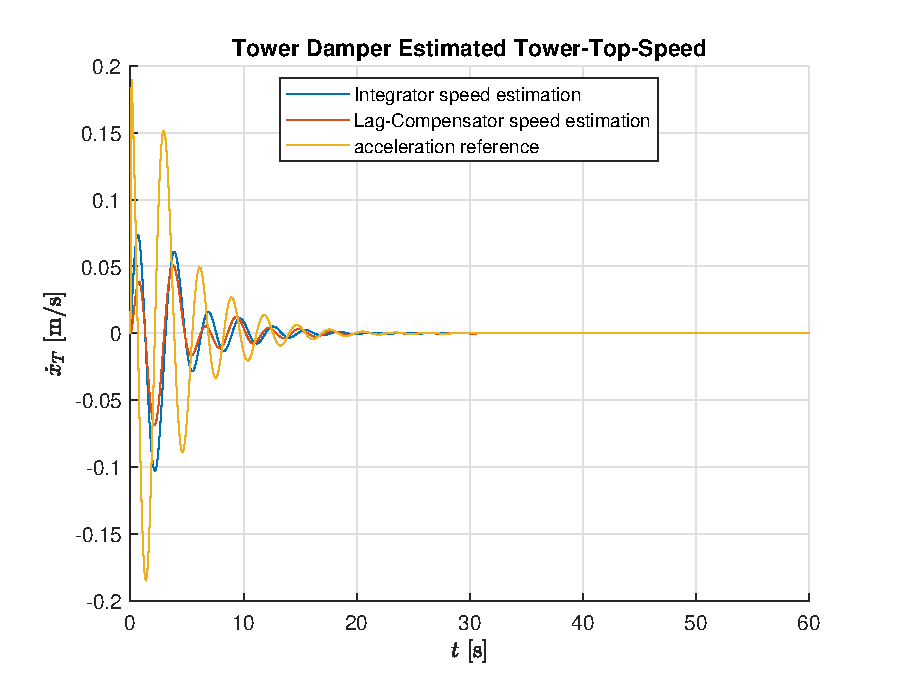
\includegraphics[width=12cm]{Figures/WindStepEst.eps}
	\caption{Tower Damper Estimated Tower-Top-Speed}
	\label{fig:TDWindStepEst}
\end{figure}
\begin{figure}[tbh]
	\centering	
	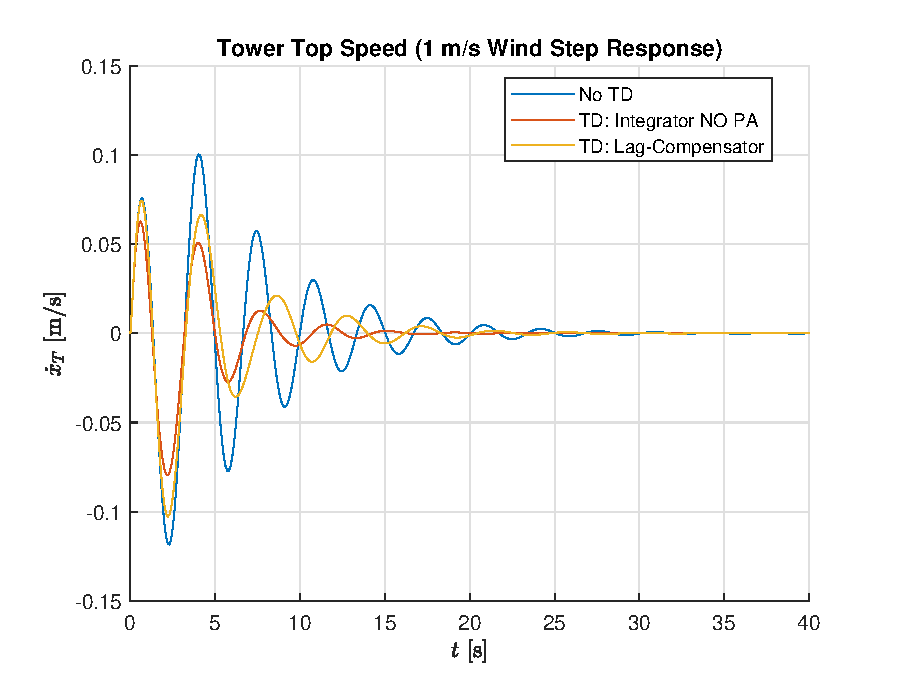
\includegraphics[width=12cm]{Figures/WindStep.eps}
	\caption{Tower-Top-Speed}
	\label{fig:TDWindStep}
\end{figure}
Both methods resulting into a damping of the tower top speed. Nevertheless the integrator method gives better result in the wind step test due to the smother damping of the oscillation. The Lag-Compensator method leads first to a faster damping but to stop the tower movement both methods are nearly equally fast. 

To further test them the SLOW-Model is disturbed with a turbulent wind field similar to the exercise in \cite{2024}. The reduction in DEL for the tower base bending moment is evaluated by tower base bending moment spectrum computed in figure \ref{fig:TDDEL}. This also shows that both methods reducing the loads at the eigenfrequency of the tower. The comparison of the damping method shows, that the Lag-Compensator has a higher damping effect at the eigenfrequency but leads to higher loads between $\SI{0.1}{Hz}$ and $\SI{0.2}{Hz}$ as well as above the eigenfrequency between $\SI{0.35}{Hz}$ and $\SI{0.55}{Hz}$. The Lag-Compensator can be tuned in such a way that the damping at the eigenfrequency is similar to the integrator method which will reduce the loads in the above mentioned frequency ranges.
\begin{figure}[tbh]
	\centering	
	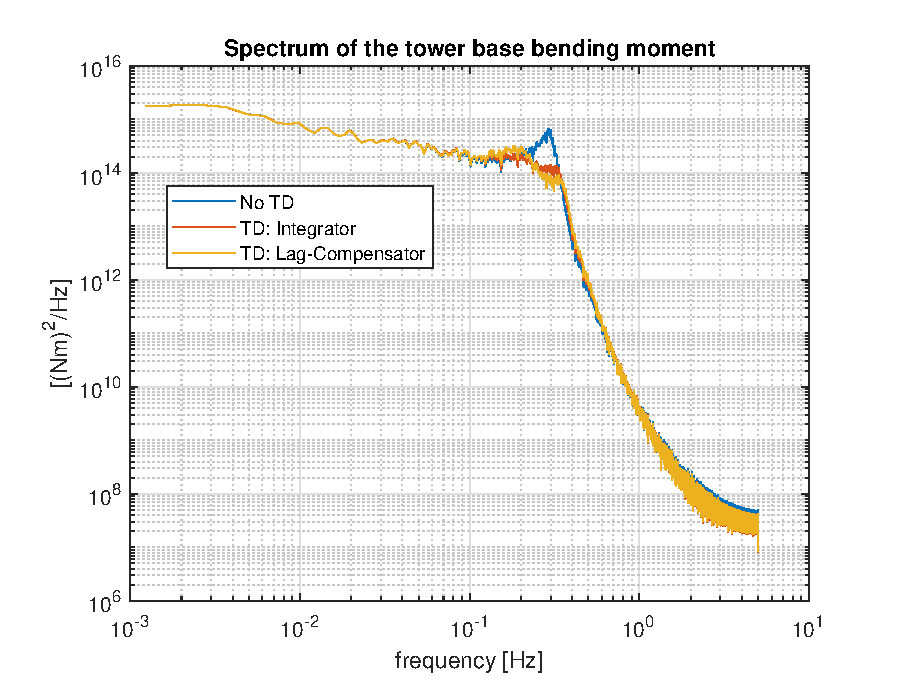
\includegraphics[width=12cm]{Figures/TDSpectrum.eps}
	\caption{Spectrum of the tower base bending moment}
	\label{fig:TDDEL}
\end{figure}      